\chapter{Introduction\label{cha:chapter1}}
\section{Context and Problem}
There is a vast variety of different object detection (OD) algorithms reaching from feature-based to template-based methods, and more recently, also deep-learning-based approaches. Especially the latter have conquered the field very rapidly and consistently improved the state of the art in many established OD benchmarks~\cite{Houben2013DetectionBenchmark},~\cite{Geiger2012AreSuite}. However, this improvement has not yet arrived at the shop floors of manufacturing companies. This is in part due to characteristics of the method, such as the large amount of required training data. Moreover, another reason is that the current machine vision infrastructure is not flexible enough to keep track of the dynamic development in the field of OD. Deploying or even only testing a new method typically requires a certain investment in cost and time that has to be justified very well. This workflow can be greatly accelerated by using service-oriented architectures (SOA)~\cite{Rudorfer2018IndustrialServices}.

A recent example of how OD can be integrated into manufacturing is depicted in figure~\ref{fig:fanuc}. A robot arm is equipped with two cameras for movement guidance. If the cylindrical objects at the bottom of the picture are to be picked, their poses have to be detected. As object detection methods (ODM) are best suited for a specific class of objects (e.g., rotationally symmetric), it is likely that with a new part type an ODM exchange is necessary. For every new object new training data has to be gathered. This is a tedious task. Moreover, the software is usually coupled tightly to the hardware, so the machine manufacturer has to be contacted for a change of software or even hardware. 
\begin{figure}[ht]
    \centering
    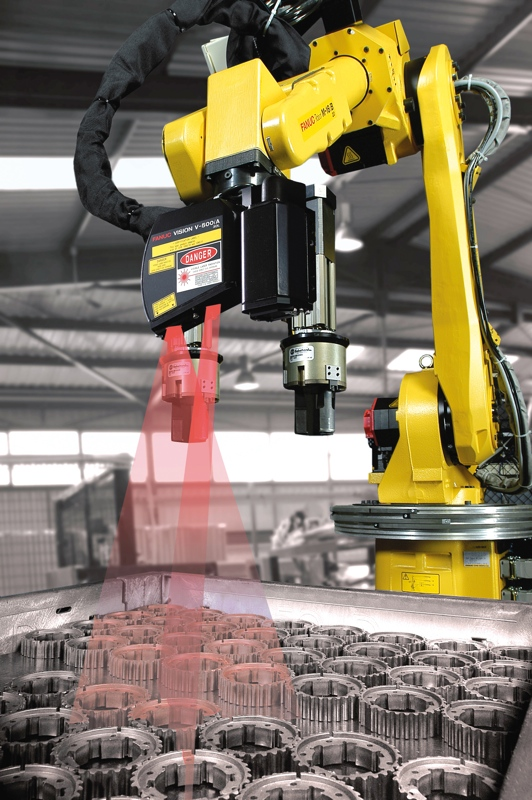
\includegraphics[width=0.4\textwidth]{img/Fanuc_iRVision.png}
    \caption{A Fanuc iRVision robot is guided by stereo-vision cameras~\cite{Gonzalez2017Smart2019}.}
    \label{fig:fanuc}
\end{figure}

Assuming a SOA is used for the robot guidance software, the main challenges are decoupling the software of the hardware, the composition of the services and meeting real-time requirements. Real-time in this context does not mean "as fast as possible" but rather "right on time", i.e., at every discrete timestep the system state must be known.

\section{Objectives}
The goal of this thesis is to simplify the process of programming an object detector and integrating it into the manufacturing process. In fact, the main objective is to avoid any programming – instead, a framework shall be proposed that allows generating an OD service from a single example image or computer-aided design (CAD) file.

The service should detect the object with a specified method and should have the appropriate interfaces for convenient integration into SOA. The key advantage is that new methods can be tested and deployed without any effort. The manufacturer can generate and deploy a service which has the same interface as the old one but uses an updated method.

The approach of this thesis is to use as many established protocols and semantic standards as possible to achieve maximum interoperability. This is the base for fast testing and deployment of new components. Ultimately, the thesis intends to create a library of reusable "plug-and-work" ODMs and other components. In this context, the open platform communication (OPC) foundation as a conglomerate of key players from different divisions in industry is of great help. It pursues vendor-independent communication between machines. As part of its work it releases semantic standards, one of which is OPC unified architecture (OPC UA) Vision~\cite{VDMA2018OPC40100-1:2018-11}. It abstracts processes in machine vision systems. While it is in draft state, this work adheres to the specification on the concept level and to some extent in the implementation. 

One central aspect of OPC UA Vision is recipe management. Recipes describe properties, procedures and parameters for a machine vision job. As they remain vendor specific in OPC UA Vision, one challenge is abstracting ODM procedures. A proposition of two general OD phases is given in this thesis.

Deployment and composition of services should also not be disregarded. Docker is used as virtualization technology and store for services. The composition is simple: camera and OD services (ODS) are called in sequence via the recipe.

\section{Delimitation}
During the design phase of a SOA-based framework (or any other software framework), numerous aspects have to be considered. Two important ones in manufacturing are safety and security~\cite{Hornberg2017HandbookVision}. They are not completely excluded in this thesis, but only considered to a very limited extent.

Also, the evaluation of the framework is not yet quantified as it is dependent on the ODM in use and moreover where the components are deployed. To thoroughly test this, a testbed inside an industrial environment must be available.

In operation technology, real-time applications are crucial~\cite{Wilmes2019ZauberwortKonvergenz}. As the framework tends to connect information and operation technology domains, it is desirable to illuminate real-time aspects, too. As of now, the standardization process for connecting both domains through, e.g., time-sensitive networking (TSN) is not advanced enough to include it in this work.

\section{Structure}
The thesis is structured as follows: The first chapter explains the problem, its relevance and outlines the objectives of the thesis. Chapter~\ref{cha:chapter2} provides the necessary background information for this work and gives an overview of recent research and related work on SOAs and OD. The pursued approaches for the proposed framework are described in detail in Chapter~\ref{cha:chapter4}. Chapter~\ref{cha:chapter5} is concerned with the implementation. It comprises the rationale of the used programming language and the explanation of the software architecture with the help of sequence, package and class diagrams. In Chapter~\ref{cha:chapter6}, an evaluation method for SOAs is introduced and applied to the framework. The results are discussed and conceptual weaknesses are considered. The thesis is concluded by Chapter~\ref{cha:chapter7}, which also points to further improvements and future research directions.